\documentclass[11pt]{article}
%-----------Packeges---------------%
\usepackage{amsmath}
\usepackage{amssymb}
\usepackage{amsfonts}
\usepackage{tocloft}
\usepackage{float}
\usepackage{graphicx}
\usepackage[bookmarks=true]{hyperref}
\usepackage{fancyhdr}


%----------Definition & Theorem----%
\newtheorem{definition}{Definition}[subsection]
\newtheorem{theorem}{Theorem}[subsection]
\newtheorem{proposition}{Proposition}[subsection]
\newtheorem{lemma}{Lemma}[subsection]
\newtheorem{corollary}{Corollary}[subsection]

\usepackage{enumerate}
\usepackage{stmaryrd}
\pagestyle{fancy}
\fancyhead[L]{Math444}
\fancyhead[C]{HW11
}
\fancyhead[R]{Lanxiao Bai}
\newcommand{\qed}{
	\begin{flushright}
		$\blacksquare$
	\end{flushright}}
\begin{document}
	\paragraph{7.1.10}\textbf{Proof:}
		Suppose $\varepsilon = 1$, and for any $\delta > 0$, if we choose tags in each partition to be irrational in $[0, 1]$, each for any $L \in \mathbb{R}$
			\[S(f; \dot{\mathcal{P})} = {\delta} \sum_{i = 0}^{1/\delta} \frac{1}{x_i}\]
			
			which does not converge since it's a p-series with $p < 1$. Hence, $g \notin \mathcal{R}[0, 1]$.
			
		However, if we choose tags in each equal partition to be rational in $[0, 1]$, and order them by the number of subintervals of the partitions, then
		\[||\dot{\mathcal{P}_n}|| = \frac{1}{n}\] converges to $0$.
		
		And \[|\lim S(f; \dot{\mathcal{P}}) - 0| = |\lim 0 ||\dot{\mathcal{P}}|| - 0| = 0 < \varepsilon\]
		
		for all $\varepsilon > 0$.
		
		Hence, by definition, 
		\[\lim S(f; \dot{\mathcal{P}}) = 0\]
		\qed
			
			
	\paragraph{7.2.2}\textbf{Proof:}
		Let $\dot{\mathcal{Q}_{n}}$ be a partition of $[0, 1]$ whose tags are all irrational, so
			\[S(h; \dot{\mathcal{Q}_n}) = 0\]
			
			for all $n$. 
						
			And if for $\dot{\mathcal{P}}$, we take all the right endpoints to be tags, then $S(h; \dot{\mathcal{P}_n})$ we have
			
			\[S(f; \dot{\mathcal{P}_n}) \geq 1 + 1 = 2\]
			
		Hence, if $\varepsilon = 2$, then for any partition with $||\dot{\mathcal{P}_n}||< \eta$ and $||\dot{\mathcal{Q}_n}||< \eta$
		
		there is always
		\[|\dot{\mathcal{P}_n} - \dot{\mathcal{Q}_n}| \geq 2 = \varepsilon\]
		
		So by Cauchy Criterion, $h$ is not integrable on $[0, 1]$.
		\qed
			
	\paragraph{7.2.4}\textbf{Proof:}
		Since for any $\varepsilon > 0$, if $x \geq \varepsilon / 2$, there is $|\omega - \alpha| = |2x| = 2x \geq \varepsilon$.
		
		Hence, this does not satisfy the requirement of Squeeze Theorem.
		\qed
		
	\paragraph{7.2.6}
		\textbf{Claim:} $\psi$ is not necessarily a step function.
		
		\textbf{Proof:} Let 
		\[\psi(x) = \begin{cases}
			1 & \text{$x$ is rational}\\
			0 & \text{otherwise} 
		\end{cases}	\]
		
		then $\psi$ only takes $2$ values. However, since $\psi$ is not in $\mathcal{R}[a, b]$ as shown in Example 7.2.2(b), by Theorem 7.2.5, $\psi$ is not a step function.
		\qed
		
	\paragraph{7.2.13}
		\textbf{Example:} $f(x) = 1/x$ is integrable in $[c, 1]$ for any $c \in [0, 1]$ but not on $[0, 1]$.
		
	\paragraph{7.2.15}\textbf{Proof:}
		Let $\mathcal{P} = \{I_i\}_{i = 1}^n$ be a partition that $||\mathcal{P}|| < \delta$, that all discontinuous points are on the endpoints of subintervals, then we have $u_i \in I_i$ to be the minimum of $I_i$ and $v_i \in I_i$ to be the maximum of $I_i$ by Maximum-minimum Theorem.
		
		Then we let $\alpha(x) = f(u_i)$ and $\omega(x) = f(v_i)$ when $x \in [x_{i - 1}, x_i)$ for $i = 0, 1, \cdots, n - 1$ and $\alpha(x) = f(u_n)$ and $\omega(x) = f(v_n)$ when $x \in [x_{n - 1}, x_n]$.
		
		Then by definition we have 
		\[\alpha(x) \leq f(x) \leq \omega(x)\]
		
		Since $f$ in each subintervals in $\mathcal{P}$ is continuous, and is uniformly continuous as a result, we have that for any $\varepsilon > 0$, there is $\delta > 0$ that when $u, v \in [a, b]$ and $0  < |u - v| < \delta$, there is
		
		\[|f(c) - f(x)| < \varepsilon/ (b - a) \]
		
		So 
		\begin{align}
			&\int_a^b (\omega(x) - \alpha(x)) = \sum_{i = 0}^{n} (f(v_i) - f(u_i))(x_{i + 1} - x_i)\nonumber\\
			&\phantom{\int_a^b (\omega(x) - \alpha(x))} < \sum_{i = 0}^{n} \frac{\varepsilon}{b - a}(x_{i} - x_{i - 1}) = \varepsilon\nonumber
		\end{align}
		
		Hence, by Squeeze Theorem, $f \in \mathcal{R}[a, b]$.
		\qed
		
		
		
	\paragraph{7.3.3}
		\begin{align}
			&\int_{-2}^3 g(x)dx = \int_{-2}^{-1} g(x)dx + \int_{-1}^{1}g(x)dx + \int_{1}^3 g(x)dx\nonumber\\
			&\phantom{\int_{-2}^3 g(x)dx} = (\frac{x^2}{2})|^{-1}_{-2} + (-\frac{x^2}{2})|^{1}_{-1} + (\frac{x^2}{2})|^{3}_{1}\nonumber\\
			&\phantom{\int_{-2}^3 g(x)dx} = \frac{1 - 4}{2} + 0 + \frac{9 - 1}{2} = \frac{5}{2}\nonumber
		\end{align}
	\paragraph{7.3.12}
		\begin{align}
			F(x) = \int_0^x f = 
			\begin{cases}
				\int^x_0 xdx = \frac{x^2}{2} & 0 \leq x < 1\\
				\int^x_0 1dx = x & 1 \leq x < 2\\
				\int^x_0 xdx = \frac{x^2}{2} & 2 \leq x < 3
			\end{cases}\nonumber
		\end{align}
		
		With sketch
		\begin{center}
			\begin{figure}[H]
			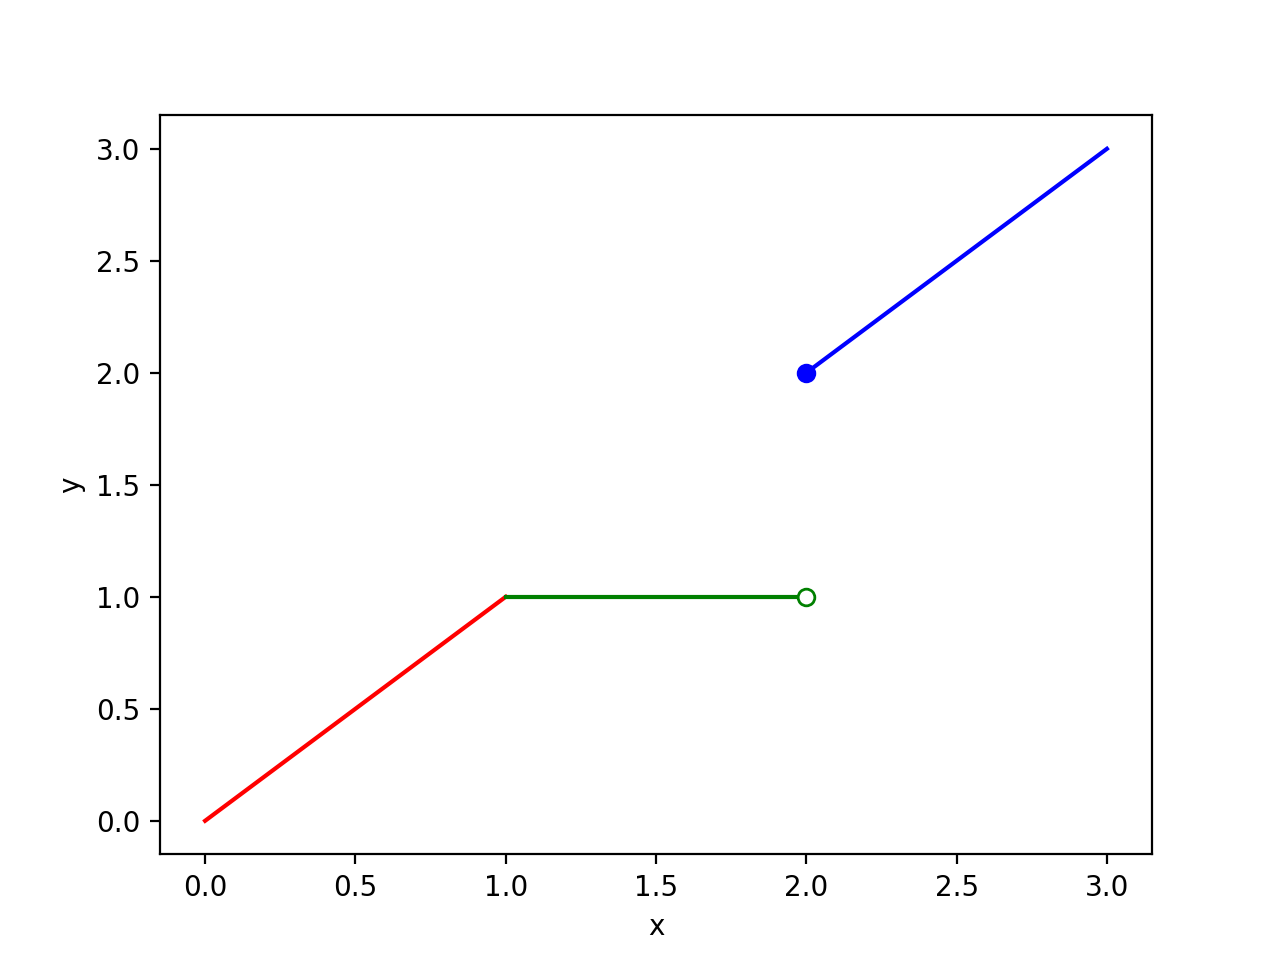
\includegraphics[width=12cm]{7_3_12_f}
			\caption{f(x)}
			\end{figure}
		\end{center}
		\begin{center}
			\begin{figure}[H]
			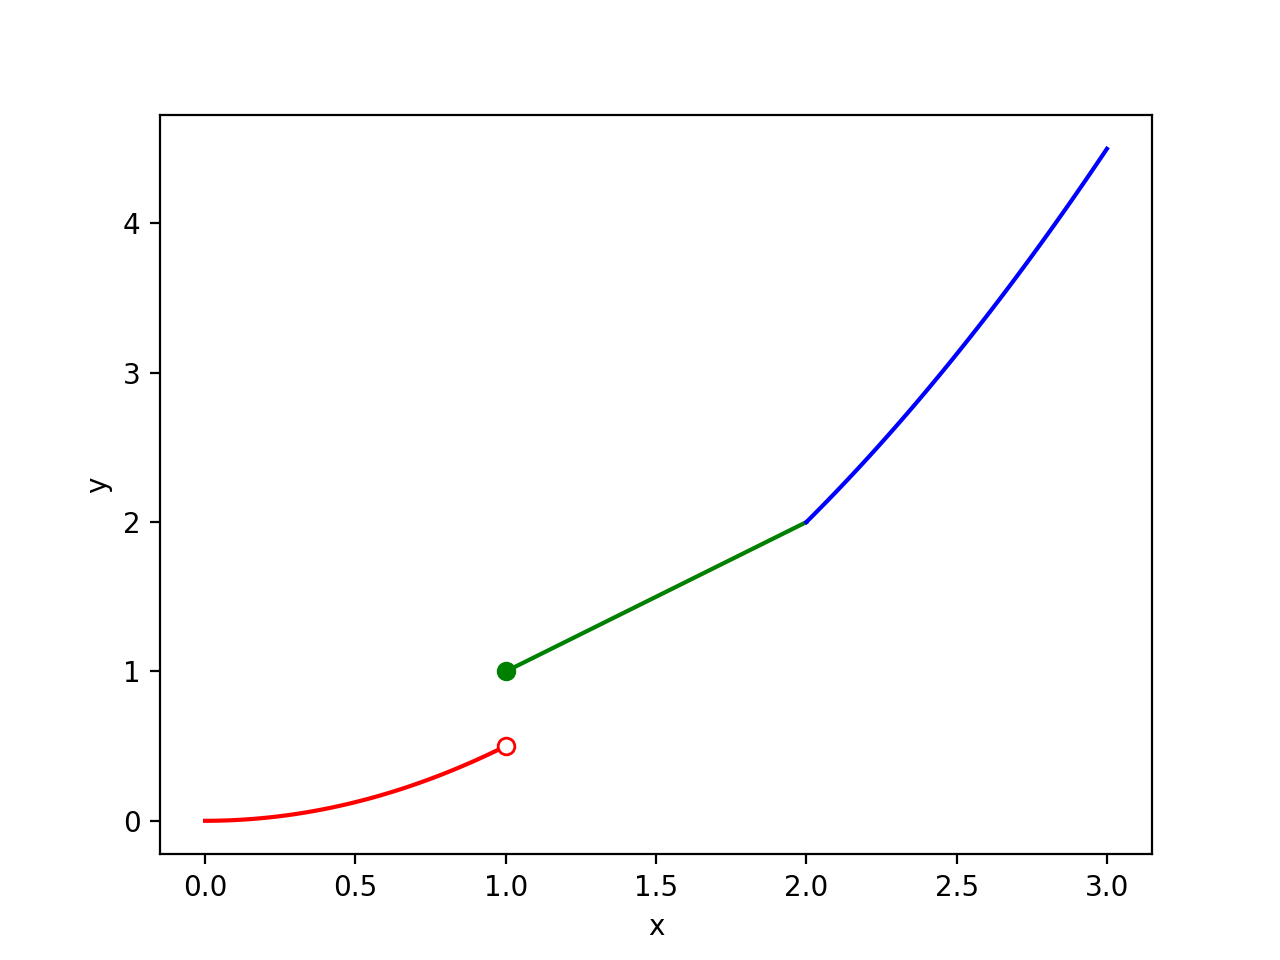
\includegraphics[width=12cm]{7_3_12}
			\caption{F(x)}
			\end{figure}
		\end{center}
		
		So $F(x)$ is differentiable in $[0, 1) \cup (1, 2) \cup (2, 3])$, and 
		\[F'(x) = \begin{cases}
			x & 0 \leq x < 1\\
			1 & 1 < x < 2\\
			x & 2 < x \leq 3
		\end{cases}	\]
\end{document}
